\documentclass[a4paper,11pt]{article}
\usepackage{titlesec}
\titleformat{\paragraph}
{\normalfont\normalsize\bfseries}{\theparagraph}{1em}{}
\titlespacing*{\paragraph}
{0pt}{3.25ex plus 1ex minus .2ex}{1.5ex plus .2ex}

\usepackage[utf8]{inputenc}
\usepackage[T1]{fontenc} % LY1 also works
\usepackage[margin=1in]{geometry}
\usepackage{tabularx}
%% Font settings suggested by fbb documentation.
\usepackage{textcomp} % to get the right copyright, etc.
\usepackage[lining,tabular]{fbb} % so math uses tabular lining figures
\usepackage[scaled=.95,type1]{cabin} % sans serif in style of Gill Sans
\usepackage[varqu,varl]{zi4}% inconsolata typewriter
\useosf % change normal text to use proportional oldstyle figures
%\usetosf would provide tabular oldstyle figures in text

\usepackage{microtype}
\usepackage{siunitx}
\DeclareSIUnit{\belmilliwatt}{Bm}
\DeclareSIUnit{\dBm}{\deci\belmilliwatt}
\sisetup{range-phrase=--, range-units=single, binary-units = true}
\usepackage{graphicx}
\usepackage{tikz}
\usepackage{svg}
%\usepackage{hyperref}
\usetikzlibrary{arrows, shadows}
\tikzset{%
  cascaded/.style = {%
    general shadow = {%
      shadow scale = 1,
      shadow xshift = -1ex,
      shadow yshift = 1ex,
      draw,
      thick,
      fill = white},
    general shadow = {%
      shadow scale = 1,
      shadow xshift = -.5ex,
      shadow yshift = .5ex,
      draw,
      thick,
      fill = white},
    fill = white, 
    draw,
    thick,
    minimum width = 1.5cm,
    minimum height = 2cm}}
    
\usepackage{enumitem}
\setitemize{noitemsep,topsep=0pt,parsep=0pt,partopsep=0pt}
\setenumerate{noitemsep,topsep=0pt,parsep=0pt,partopsep=0pt}
\setlist{leftmargin=*}
\usepackage{listings}
\lstset{
	basicstyle=\ttfamily,
	frame=single,
	breaklines=true,
	morecomment=[l][\color{green}]{\#},
}
\usepackage[os=win]{menukeys}
\renewmenumacro{\keys}[+]{shadowedroundedkeys}

\usepackage{booktabs,caption}
\usepackage{threeparttable}
\newcolumntype{L}[1]{>{\raggedright\let\newline\\\arraybackslash\hspace{0pt}}m{#1}}
\newcolumntype{C}[1]{>{\centering\let\newline\\\arraybackslash\hspace{0pt}}m{#1}}
\newcolumntype{R}[1]{>{\raggedleft\let\newline\\\arraybackslash\hspace{0pt}}m{#1}}
\usepackage{tabularx} 

\usepackage{multirow}
\usepackage{longtable,booktabs,threeparttablex}

\usepackage{stackengine}
\usepackage{scalerel}
\usepackage{xcolor,mdframed}

\newcommand\danger[1][5ex]{%
  \renewcommand\stacktype{L}%
  \scaleto{\stackon[1.3pt]{\color{red}$\triangle$}{\tiny !}}{#1}%
}

\newenvironment{important}[1][]{%
   \begin{mdframed}[%
      backgroundcolor={red!15}, hidealllines=true,
      skipabove=0.7\baselineskip, skipbelow=0.7\baselineskip,
      splitbottomskip=2pt, splittopskip=4pt, #1]%
   \makebox[0pt]{% ignore the withd of !
      \smash{% ignor the height of !
         %\fontsize{32pt}{32pt}\selectfont% make the ! bigger
         \hspace*{-45pt}% move ! to the left
         \raisebox{-5pt}{% move ! up a little
            {\danger}% type the bold red !
         }%
      }%
   }%
}{\end{mdframed}}

\newcommand\info[1][5ex]{%
  \renewcommand\stacktype{L}%
  \scaleto{\stackon[1.2pt]{\color{blue}$\bigcirc$}{\raisebox{-1.5pt}{\small i}}}{#1}%
}

\newenvironment{information}[1][]{%
   \begin{mdframed}[%
      backgroundcolor={blue!15}, hidealllines=true,
      skipabove=0.7\baselineskip, skipbelow=0.7\baselineskip,
      splitbottomskip=2pt, splittopskip=4pt, #1]%
   \makebox[0pt]{% ignore the withd of !
      \smash{% ignor the height of !
         %\fontsize{32pt}{32pt}\selectfont% make the ! bigger
         \hspace*{-45pt}% move ! to the left
         \raisebox{-5pt}{% move ! up a little
            {\info}% type the bold red !
         }%
      }%
   }%
}{\end{mdframed}}

\pgfdeclarelayer{background}
\pgfdeclarelayer{foreground}
\pgfsetlayers{background,main,foreground}

\newcommand{\bitrect}[2]{
  \begin{pgfonlayer}{foreground}
    \draw [thick] (0,0) rectangle (#1,1);
    \pgfmathsetmacro\result{#1-1}
    \foreach \x in {1,...,\result}
      \draw [thick] (\x,1) -- (\x, 0.8);
  \end{pgfonlayer}
%  \node [below left, align=right] at (0,0) {Type \\ Reset};
  \bitlabels{#1}{#2}
}
\newcommand{\rwbits}[3]{
  \draw [thick] (#1,0) rectangle ++(#2,1) node[pos=0.5]{#3};
  \pgfmathsetmacro\start{#1+0.5}
  \pgfmathsetmacro\finish{#1+#2-0.5}
%  \foreach \x in {\start,...,\finish}
%    \node [below, align=center] at (\x, 0) {R/W \\ 0};
}
\newcommand{\robits}[3]{
  \begin{pgfonlayer}{background}
    \draw [thick, fill=lightgray] (#1,0) rectangle ++(#2,1) node[pos=0.5]{#3};
  \end{pgfonlayer}
  \pgfmathsetmacro\start{#1+0.5}
  \pgfmathsetmacro\finish{#1+#2-0.5}
%  \foreach \x in {\start,...,\finish}
%    \node [below, align=center] at (\x, 0) {RO \\ 0};
}
\newcommand{\bitlabels}[2]{
  \foreach \bit in {1,...,#1}{
     \pgfmathsetmacro\result{#2}
     \node [above] at (\bit-0.5, 1) {\pgfmathprintnumber{\result}};
   }
}

\usepackage{makecell}
\usepackage{hyperref}
\newcommand{\vna}{LibreVNA}

\title{LibreVNA USB Protocol\\\small{Version 12}}

\begin{document}
\maketitle
\tableofcontents
\clearpage

\section{USB device}
The LibreVNA implements a ``custom class'' USB device. It uses a VID of 0x0483 and a PID of 0x4121. The custom class contains a single interface with three bulk endpoints:
\begin{itemize}
\item \textbf{Endpoint 0x01:} Communication data from the USB host to the LibreVNA
\item \textbf{Endpoint 0x81:} Communication data from the LibreVNA to the USB host
\item \textbf{Endpoint 0x82:} Debug messages from the LibreVNA
\end{itemize}

Endpoint 0x82 is exclusively used for debug messages. They are transmitted in ASCII format. All protocol packets described in this document are always transmitted over endpoints 0x01 and 0x81.

\section{General packet structure}
The USB traffic through bulk endpoints can be viewed as a stream of bytes. The communication between the LibreVNA and the USB host is done in packets. To detect the packets within the data stream, some framing is needed. This general package structure is described in this section.

Each packet consists of the following fields:
\begin{enumerate}
\item \textbf{Header:} 1 byte, always 0x5A
\item \textbf{Length:} 2 bytes, length of the overall packet in bytes, including the header and the checksum
\item \textbf{Type:} 1 byte, defines the type of packet and subsequently the data encoding within the payload
\item \textbf{Payload:} Any amount of bytes, content depends on the packet type
\item \textbf{CRC:} 4 bytes, CRC32 over all other packet bytes (header, length, type and payload)
\end{enumerate}
\noindent
All values in the USB protocol are little-endian.

\section{Packet types}
The following packet types are available:
\begin{ThreePartTable}
\setlength\tabcolsep{3pt}

\begin{TableNotes}
  \item[a] Direction of packet transfer:
  \begin{footnotesize}
  \begin{itemize}
  \item \textbf{D$\rightarrow$H:} Device to host
  \item \textbf{H$\rightarrow$D:} Host to device
  \item \textbf{D$\leftrightarrow$H:} Both directions used
  \end{itemize}
  \end{footnotesize}
  \item[b] Packet type that will be sent in response to this packet
  \item[c] The response will be sent multiple times
\end{TableNotes}

\begin{longtable}{p{0.06\textwidth} |  p{0.3\textwidth} | p{0.07\textwidth} | p{0.4\textwidth} |p{0.1\textwidth} }
\toprule
\textbf{Type} &\textbf{Name}  & \textbf{Dir}\tnote{a} &\textbf{Description} &\textbf{Answer}\tnote{a} \\ 
\hline
\endhead
\midrule[\heavyrulewidth]
\endfoot  
\midrule[\heavyrulewidth]
\insertTableNotes  % tell LaTeX where to insert the table-related notes
\endlastfoot

2 & SweepSettings & H$\rightarrow$D & Sets the sweep paramaters and starts the sweep in VNA mode& 27\tnote{c}\\
3 & ManualStatusV1 & D$\rightarrow$H & Contains the hardware status when in manual control mode & None\\
4 & ManualControlV1 & H$\rightarrow$D & Transfers the manual control configuration, switches the device into manual control mode & 3\tnote{c}\\
5 & DeviceInfo & D$\rightarrow$H & Contains the device information (firmware/hardware version, capabilities,...)&None \\
6 & FirmwarePacket & H$\rightarrow$D & Contains a piece of firmware data &None \\
7 & Ack & D$\rightarrow$H & Sent as a response to every successfully received and handled packet&None \\
8 & ClearFlash & H$\rightarrow$D & Triggers the flash erase procedure. Must be issues before transferring firmware data&None \\
9 & PerformFirmwareUpdate & H$\rightarrow$D & Triggers the firmware update once all firmware data has been transferred&None \\
10 & Nack & D$\rightarrow$H & Sent as a response to every unknown command or failure to execute the requested command&None \\
11 & Reference & H$\rightarrow$D & Configure the external/internal reference &None \\
12 & Generator & H$\rightarrow$D & Switches the VNA into generator mode and configures the generator output&None \\
13 & SpectrumAnalyzerSettings & H$\rightarrow$D & Sets the sweep parameters and starts the sweep in spectrum analyzer mode&14\tnote{c} \\
14 & SpectrumAnalyzerResult & D$\rightarrow$H & Sent for every sampled frequency within the sweep in spectrum analyzer mode&None \\
15 & RequestDeviceInfo & H$\rightarrow$D & Makes the device send the DeviceInfo packet &5 \\
16 & RequestSourceCal & H$\rightarrow$D & Makes the device send the source calibration packets & 18\tnote{c}\\
17 & RequestReceiverCal & H$\rightarrow$D & Makes the device send the receiver calibration packets & 19\tnote{c}\\
18 & SourceCalPoint & D$\leftrightarrow$H & Contains a single source amplitude calibration point &None\\
19 & ReceiverCalPoint & D$\leftrightarrow$H & Contains a single receiver amplitude calibration point &None \\
20 & SetIdle & H$\rightarrow$D & Stops all device activity & None \\
21 & RequestFrequencyCorrection & H$\rightarrow$D & Makes the device send the frequency calibration packet &22 \\
22 & FrequencyCorrection & D$\leftrightarrow$H & Contains the frequency calibration factor & None\\
23 & RequestAcquisition-FrequencySettings & H$\rightarrow$D & Makes the device send the acquisition frequency settings & 24\\
24 & AcquisitionFrequencySettings & D$\rightarrow$H & Contains the configuration of IF and sample frequencies &None \\
25 & DeviceStatusV1 & D$\rightarrow$H & Contains the hardware device status (lock, temperatures,...) &None \\
26 & RequestDeviceStatus & H$\rightarrow$D & Makes the device send the device status &25 \\
27 & VNADatapoint & D$\rightarrow$H & Sent for every sampled frequency within the sweep in VNA mode &None \\
28 & SetTrigger & D$\leftrightarrow$H & Updates the trigger status for synchronization over USB & None\\
29 & ClearTrigger & D$\leftrightarrow$H & Updates the trigger status for synchronization over USB & None\\
\end{longtable}   
\end{ThreePartTable}
An Ack is transmitted by the device for every received command after it has been handled successfully. If additional responses are triggered by the command, they are transmitted after this Ack.

Received packets from the device are not acknowledged by the host; the host never sends an Ack packet.

\subsection{SweepSettings}
Transmitting this packet will switch the LibreVNA into VNA mode and start the sweep. During the sweep, VNADatapoint packets are generated for each completed point in the sweep.

The sampling for each frequency (or power) point in the sweep is done in stages. In each stage, the stimulus can be active at another port. A typical full two-port sweep would therefore use two stages, with the stimulus being active on port 1 during stage 0 and on port 2 during stage 1. For faster measurements, this could be reduced to a single stage if only a subset of the S-parameters is required. Similarly, more than two stages can be used (with the stimulus inactive during some) when multiple devices are synchronized. Another device in the setup will have to generate the stimulus during the inactive stages.


The packet contains the following fields:
\begin{ThreePartTable}
\setlength\tabcolsep{3pt}

\begin{longtable}{p{0.08\textwidth} |  p{0.08\textwidth}  |  p{0.1\textwidth}| p{0.25\textwidth} | p{0.43\textwidth}}
\toprule
\textbf{Offset} &\textbf{Length} &\textbf{Type} & \textbf{Name} &\textbf{Description} \\ 
\hline
\endhead
\midrule[\heavyrulewidth]
\endfoot  
\midrule[\heavyrulewidth]
%\insertTableNotes  % tell LaTeX where to insert the table-related notes
\endlastfoot

0 & 8 & UINT64 & f\_start & Start frequency in Hz \\
8 & 8 & UINT64 & f\_stop & Stop frequency in Hz \\
16 & 2 & UINT16 & points & Number of points in the sweep \\
18 & 4 & UINT32 & IF\_bandwidth & Bandwidth of the IF sampling in Hz \\
22 & 2 &  INT16 &cdbm\_excitation\_start &  Stimulus power at the first point in $\frac{1}{100}$dBm \\
24 & 2 & UINT16 & Configuration & Bitmap for configuration, see below \\
26 & 2 &  INT16 &cdbm\_excitation\_stop & Stimulus power at the last point in $\frac{1}{100}$dBm \\
\end{longtable}   
\end{ThreePartTable}

\paragraph{Configuration:}
\begin{center}
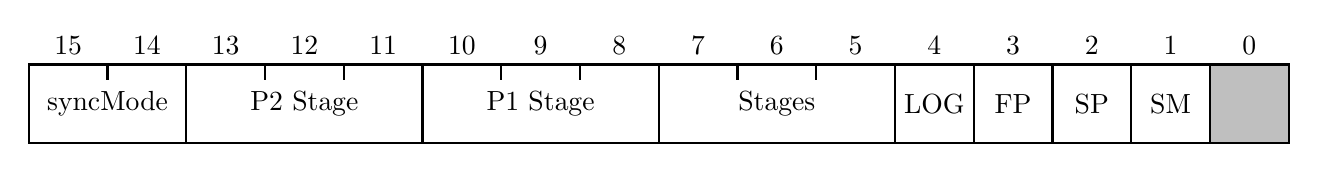
\begin{tikzpicture}
\bitrect{16}{16-\bit}
\rwbits{0}{2}{syncMode}
\rwbits{2}{3}{P2 Stage}
\rwbits{5}{3}{P1 Stage}
\rwbits{8}{3}{Stages}
\rwbits{11}{1}{LOG}
\rwbits{12}{1}{FP}
\rwbits{13}{1}{SP}
\rwbits{14}{1}{SM}
\robits{15}{1}{}
\end{tikzpicture}
\end{center}
\begin{itemize}
\item \textbf{syncMode:} Synchronization mode when multiple devices are used together
\begin{center}
\begin{tabular}{ c|c }
Setting & Synchronization\\
 \hline
00 & Disabled \\
01 & USB\\
10 & External reference\\
11 & External trigger\\
\end{tabular}
\end{center}
\item \textbf{P1 Stage:} Sets the stage number when the stimulus is active at port 1. Stage number indizes start at 0.
\item \textbf{P2 Stage:} Sets the stage number when the stimulus is active at port 2. Stage number indizes start at 0.
\item \textbf{Stages:} Sets the number of used stages. The number of stages is one more than this value. E.g. set to 1 for 2 stages
\item \textbf{LOG:} Set for a logarithmic sweep (only for frequency, power adjustment during the sweep is always linear)
\item \textbf{FP:} Fixed power setting. This must be enabled for power sweeps (when  cdbm\_excitation\_start $\neq$  cdbm\_excitation\_stop)
\begin{center}
\begin{tabularx}{\textwidth}{ c|X }
Setting & Behavior\\
 \hline
0 & Attenuator setting is fixed during the sweep. This will result in inaccurate stimulus level but prevent discrete jumps in output power. \\
1 & Attenuator setting is changed during the sweep. This will result in more accurate stimulus level but also create discrete jumps in output power. \\
\end{tabularx}
\end{center}
\item \textbf{SP:} Suppress peaks. Recommended setting: always enabled.
\begin{center}
\begin{tabularx}{\textwidth}{ c|X }
Setting & Behavior\\
 \hline
0 & 2.LO is adjusted to compensate for limited frequency resolution in 1.LO. Slight decrease in maximum sweep speed. \\
1 & 2.LO is kept at its nominal value. Slightly faster sweep but this will result in peaks at frequencies where the 1.LO it too far off the ideal frequency. \\
\end{tabularx}
\end{center}
\item \textbf{SM:} Sync Master. Must be set to 1 at exactly one device when multiple devices are synchronized. Set to 0 when synchronization is disabled.
\end{itemize}

\subsection{ManualStatusV1}
This packet is generated by the LibreVNA 1.0 when in manual control mode. It is transmitted in regular intervals on its own.

The packet contains the following fields:
\begin{ThreePartTable}
\setlength\tabcolsep{3pt}

\begin{longtable}{p{0.08\textwidth} |  p{0.08\textwidth}  |  p{0.1\textwidth}| p{0.15\textwidth} | p{0.53\textwidth}}
\toprule
\textbf{Offset} &\textbf{Length} &\textbf{Type} & \textbf{Name} &\textbf{Description} \\ 
\hline
\endhead
\midrule[\heavyrulewidth]
\endfoot  
\midrule[\heavyrulewidth]
%\insertTableNotes  % tell LaTeX where to insert the table-related notes
\endlastfoot

0 & 2 & INT16 & port1min & Minimum value of the ADC at port 1 \\
2 & 2 & INT16 & port1max & Maximum value of the ADC at port 1 \\
4 & 2 & INT16 & port2min & Minimum value of the ADC at port 2 \\
6 & 2 & INT16 & port2max & Maximum value of the ADC at port 2 \\
8 & 2 & INT16 & refmin & Minimum value of the ADC at the reference receiver \\
10 & 2 & INT16 & refmax & Maximum value of the ADC at the reference receiver \\
12 & 4 & FLOAT & port1real & Real part of the complex signal at port 1 \\
16 & 4 & FLOAT & port1imag & Imaginary part of the complex signal at port 1 \\
20 & 4 & FLOAT & port2real & Real part of the complex signal at port 2 \\
24 & 4 & FLOAT & port2imag & Imaginary part of the complex signal at port 2 \\
28 & 4 & FLOAT & refreal & Real part of the complex signal at the reference receiver \\
32 & 4 & FLOAT & refimag & Imaginary part of the complex signal at the reference receiver \\
36 & 1 & UINT8 & temp\_source & Temperature of the source PLL in \si{\celsius} \\
37 & 1 & UINT8 & temp\_LO & Temperature of the LO PLL in \si{\celsius} \\
38 & 1 & UINT8 & Lock status & Bit 0: lock status of source PLL. Bit 1: lock status of LO PLL \\
\end{longtable}   
\end{ThreePartTable}

\subsection{ManualControlV1}
This packet switches the LibreVNA to manual control mode. As long as the manual control mode is active, the LibreVNA will generate ManualStatusV1 packets and send them to the host.

The packet contains the following fields:
\begin{ThreePartTable}
\setlength\tabcolsep{3pt}

\begin{longtable}{p{0.08\textwidth} |  p{0.08\textwidth}  |  p{0.1\textwidth}| p{0.25\textwidth} | p{0.43\textwidth}}
\toprule
\textbf{Offset} &\textbf{Length} &\textbf{Type} & \textbf{Name} &\textbf{Description} \\ 
\hline
\endhead
\midrule[\heavyrulewidth]
\endfoot  
\midrule[\heavyrulewidth]
%\insertTableNotes  % tell LaTeX where to insert the table-related notes
\endlastfoot

0 & 1 & UINT8 & Source High Config & Configuration of the highband source \\
1 & 8 & UINT64 & Source High Frequency & Frequency of the highband source in Hz \\
9 & 1 & UINT8 & Source Low Config & Configuration of the lowband source \\
10 & 4 & UINT32 & Source High Frequency & Frequency of the highband source in Hz \\
14 & 2 & UINT16 & Source Path Config & Configuration of the source signal from the PLLs to the ports \\
16 & 1 & UINT8 & 1.LO Config & Configuration of the 1.LO \\
17 & 8 & UINT64 & 1.LO Frequency & Frequency of the 1.LO in Hz \\
25 & 1 & UINT8 & 2.LO Enable & Set to 1 to enable the 2.LO. Set to 0 to disable the 2.LO \\
26 & 4 & UINT32 & 2.LO Frequency & Frequency of the 2.LO in Hz \\
\hline
30 & 1 & UINT8 & Receiver enable & \makecell[l]{Bit 0: Enable port 1 receiver\\Bit 1: Enable port 1 receiver\\Bit 2: Enable reference receiver} \\
\hline
31 & 4 & UINT32 & Samples & Number of ADC samples for each complex wave calculation \\
32 & 1 & UINT8 & WindowType & Window selection for the complex wave calculation \\
\end{longtable}   
\end{ThreePartTable}

\paragraph{Source High Config:}
\begin{center}
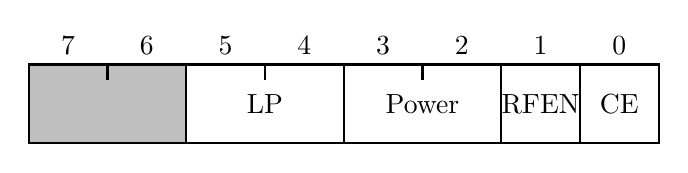
\begin{tikzpicture}
\bitrect{8}{8-\bit}
\robits{0}{2}{}
\rwbits{2}{2}{LP}
\rwbits{4}{2}{Power}
\rwbits{6}{1}{RFEN}
\rwbits{7}{1}{CE}
\end{tikzpicture}
\end{center}

\begin{itemize}
\item \textbf{LP:} Lowpass setting
\begin{center}
\begin{tabular}{ c|c }
Setting & Cut-off frequency\\
 \hline
00 & \SI{947}{\mega\hertz} \\
01 &  \SI{1.88}{\giga\hertz}\\
10 & \SI{3.5}{\giga\hertz}\\
11 & No filter\\
\end{tabular}
\end{center}
\item \textbf{Power:} Power output of the highband source PLL
\begin{center}
\begin{tabular}{ c|c }
Setting & Power\\
 \hline
00 & \SI{-4}{\dBm} \\
01 & \SI{-1}{\dBm}\\
10 & \SI{2}{\dBm}\\
11 &  \SI{5}{\dBm}\\
\end{tabular}
\end{center}
\item \textbf{RFEN:} RF output enable
\item \textbf{CE:} Chip enable
\end{itemize}

\paragraph{Source Low Config:}
\begin{center}
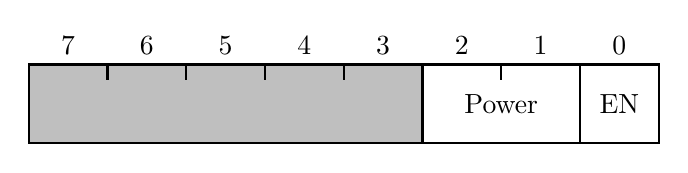
\begin{tikzpicture}
\bitrect{8}{8-\bit}
\robits{0}{5}{}
\rwbits{5}{2}{Power}
\rwbits{7}{1}{EN}
\end{tikzpicture}
\end{center}

\begin{itemize}
\item \textbf{Power:} Power output of the lowband source PLL
\begin{center}
\begin{tabular}{ c|c }
Setting & Drive Strength\\
 \hline
00 & \SI{2}{\milli\ampere} \\
01 & \SI{4}{\milli\ampere}\\
10 & \SI{6}{\milli\ampere}\\
11 &  \SI{8}{\milli\ampere}\\
\end{tabular}
\end{center}
\item \textbf{EN:} Lowband source enable
\end{itemize}

\paragraph{Source Path Config:}
\begin{center}
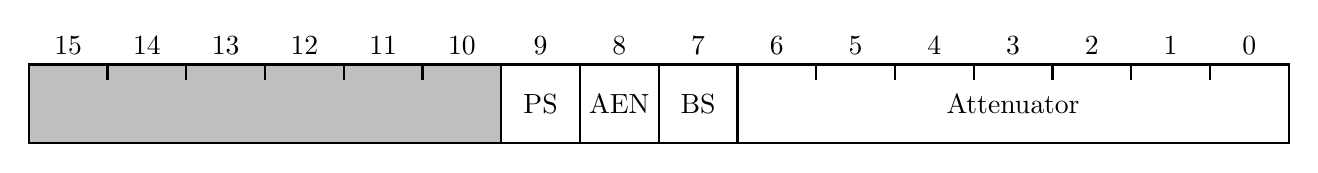
\begin{tikzpicture}
\bitrect{16}{16-\bit}
\robits{0}{6}{}
\rwbits{6}{1}{PS}
\rwbits{7}{1}{AEN}
\rwbits{8}{1}{BS}
\rwbits{9}{7}{Attenuator}
\end{tikzpicture}
\end{center}

\begin{itemize}
\item \textbf{PS:} Port switch. Set to 1 to route the source signal to port 2, set to 0 to route the source signal to port 1.
\item \textbf{AEN:} Amplifier enable.
\item \textbf{PS:} Band select. Set to 1 to use the highband source, set to 0 to use the lowband source.
\item \textbf{Attenuator:} Attenuation of the source signal in \SI{0.25}{\dBm}.
\end{itemize}

\paragraph{1.LO Config:}
\begin{center}
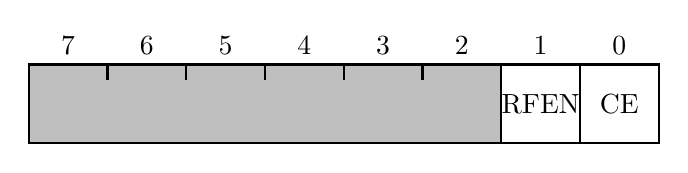
\begin{tikzpicture}
\bitrect{8}{8-\bit}
\robits{0}{6}{}
\rwbits{6}{1}{RFEN}
\rwbits{7}{1}{CE}
\end{tikzpicture}
\end{center}

\begin{itemize}
\item \textbf{RFEN:} RF output enable
\item \textbf{CE:} Chip enable
\end{itemize}

\paragraph{WindowType:}
\begin{center}
\begin{tabular}{ c|c }
Setting & Window\\
 \hline
0 & None \\
1 & Kaiser\\
2 & Hann\\
3 & Flattop\\
\end{tabular}
\end{center}

\subsection{DeviceInfo}
This packet contains information about the connected device. It can be requested by sending a RequestDeviceInfo packet. This request is the first thing that should happen after the device has been enumerated to make sure the right protocol version is used.

The packet contains the following fields:
\begin{ThreePartTable}
\setlength\tabcolsep{3pt}

\begin{longtable}{p{0.08\textwidth} |  p{0.08\textwidth}  |  p{0.1\textwidth}| p{0.25\textwidth} | p{0.43\textwidth}}
\toprule
\textbf{Offset} &\textbf{Length} &\textbf{Type} & \textbf{Name} &\textbf{Description} \\ 
\hline
\endhead
\midrule[\heavyrulewidth]
\endfoot  
\midrule[\heavyrulewidth]
%\insertTableNotes  % tell LaTeX where to insert the table-related notes
\endlastfoot

0 & 2 & UINT16 & ProtocolVersion & Set to 12. If another value is reported, refer to the corresponding protocol description.\\
2 & 1 & UINT8 & FW\_major & Major firmware version \\
3 & 1 & UINT8 & FW\_minor & Minor firmware version \\
4 & 1 & UINT8 & FW\_patch & Patch of the firmware version \\
5 & 1 & UINT8 & hardware\_version & Version of the hardware, currently only  `1' \\
6 & 1 & CHAR & HW\_revision & Revision of the hardware, currently only `B' is used \\
7 & 8 & UINT64 & MinFreq & Minimum supported frequency in Hz \\
15 & 8 & UINT64 & MaxFreq & Maximum supported frequency in Hz \\
23 & 4 & UINT64 & MinIFBW & Minimum supported IF bandwidth in Hz \\
27 & 4 & UINT64 & MaxIFBW & Maximum supported IF bandwidth in Hz \\
31 & 2 & UINT16 & MaxPoints & Maximum number of points per sweep \\
33 & 2 & INT16 & MincdBm & Minimum stimulus power in $\frac{1}{100}$dBm \\
35 & 2 & INT16 & MaxcdBm & Maximum stimulus power in $\frac{1}{100}$dBm \\
37 & 4 & UINT32 & MinRBW & Minimum supported resolution bandwidth in Hz \\
41 & 4 & UINT32 & MaxRBW & Maximum supported resolution bandwidth in Hz \\
45 & 1 & UINT8 & MaxAmplitudePoints & Maximum supported number of amplitude calibration points \\
46 & 8 & UINT64 & MaxHarmonicFrequency & Maximum supported frequency when using harmonic mixing \\
\end{longtable}   
\end{ThreePartTable}

\subsection{FirmwarePacket}
This packet contains a part of the firmware. When updating the firmware, this packet must be transmitted multiple times until the whole firmware has been transferred.

The packet contains the following fields:
\begin{ThreePartTable}
\setlength\tabcolsep{3pt}

\begin{longtable}{p{0.08\textwidth} |  p{0.08\textwidth}  |  p{0.1\textwidth}| p{0.25\textwidth} | p{0.43\textwidth}}
\toprule
\textbf{Offset} &\textbf{Length} &\textbf{Type} & \textbf{Name} &\textbf{Description} \\ 
\hline
\endhead
\midrule[\heavyrulewidth]
\endfoot  
\midrule[\heavyrulewidth]
%\insertTableNotes  % tell LaTeX where to insert the table-related notes
\endlastfoot

0 & 4 & UINT32 & Address & Address at which the firmware data starts\\
4 & 256 & UINT8 & Data & Binary firmware data \\
\end{longtable}   
\end{ThreePartTable}

\subsection{Ack}
This packet is sent by the device whenever a valid packet has been received. It has no payload.

\subsection{ClearFlash}
This packet must be sent before transferring the first piece of firmware data. It has no payload.

\subsection{PerformFirmwareUpdate}
This packet must be sent after the complete firmware data has been transmitted. It triggers the actual update process. The device will reboot during the update process. It has no payload.

\subsection{Nack}
This packet is sent by the device whenever an error occured while processing a received packet. It has no payload.

\subsection{Reference}
This packet is used to configure the external reference input and output.

The packet contains the following fields:
\begin{ThreePartTable}
\setlength\tabcolsep{3pt}

\begin{longtable}{p{0.08\textwidth} |  p{0.08\textwidth}  |  p{0.1\textwidth}| p{0.21\textwidth} | p{0.47\textwidth}}
\toprule
\textbf{Offset} &\textbf{Length} &\textbf{Type} & \textbf{Name} &\textbf{Description} \\ 
\hline
\endhead
\midrule[\heavyrulewidth]
\endfoot  
\midrule[\heavyrulewidth]
%\insertTableNotes  % tell LaTeX where to insert the table-related notes
\endlastfoot

0 & 4 & UINT32 & OutputFrequency & Frequency of the external reference output. Not every frequency can be reached by the PLL. Set to 0 to disable the reference output.\\
4 & 1 & UINT8 & ExternalInputConfig & \makecell[l]{Bit 0: Switch to external when signal detected\\Bit 1: Force usage of the external reference} \\
\end{longtable}   
\end{ThreePartTable}

\subsection{Generator}
This packet switches the LibreVNA into signal generator mode and configures the output signal.

The packet contains the following fields:
\begin{ThreePartTable}
\setlength\tabcolsep{3pt}

\begin{longtable}{p{0.08\textwidth} |  p{0.08\textwidth}  |  p{0.1\textwidth}| p{0.25\textwidth} | p{0.43\textwidth}}
\toprule
\textbf{Offset} &\textbf{Length} &\textbf{Type} & \textbf{Name} &\textbf{Description} \\ 
\hline
\endhead
\midrule[\heavyrulewidth]
\endfoot  
\midrule[\heavyrulewidth]
%\insertTableNotes  % tell LaTeX where to insert the table-related notes
\endlastfoot

0 & 8 & UINT64 & OutputFrequency & Output frequency of the generator in Hz\\
8 & 2 & INT16 & cdBmLevel & Output level in $\frac{1}{100}$dBm \\
10 & 1 & UINT8 & Configuration & Configuration bitmap, see below \\
\end{longtable}   
\end{ThreePartTable}

\paragraph{Configuration:}
\begin{center}
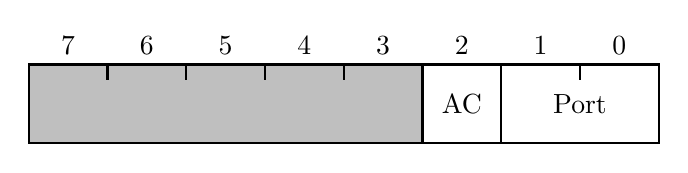
\begin{tikzpicture}
\bitrect{8}{8-\bit}
\robits{0}{5}{}
\rwbits{5}{1}{AC}
\rwbits{6}{2}{Port}
\end{tikzpicture}
\end{center}

\begin{itemize}
\item \textbf{AC:} Amplitude correction enable. If set to 1, the source amplitude calibration is used to reach better amplitude accuracy.
\item \textbf{Port:} Port selection:
\begin{center}
\begin{tabular}{ c|c }
Setting & Window\\
 \hline
0 & Disabled \\
1 & Output on port 1\\
2 & Output on port 2\\
\end{tabular}
\end{center}
\end{itemize}

\subsection{SpectrumAnalyzerSettings}
Transmitting this packet will switch the LibreVNA into spectrum analyzer mode and start the sweep. During the sweep, SpectrumAnalyzerResult packets are generated for each completed point in the sweep.

The packet contains the following fields:
\begin{ThreePartTable}
\setlength\tabcolsep{3pt}

\begin{longtable}{p{0.08\textwidth} |  p{0.08\textwidth}  |  p{0.1\textwidth}| p{0.25\textwidth} | p{0.43\textwidth}}
\toprule
\textbf{Offset} &\textbf{Length} &\textbf{Type} & \textbf{Name} &\textbf{Description} \\ 
\hline
\endhead
\midrule[\heavyrulewidth]
\endfoot  
\midrule[\heavyrulewidth]
%\insertTableNotes  % tell LaTeX where to insert the table-related notes
\endlastfoot

0 & 8 & UINT64 & f\_start & Start frequency in Hz \\
8 & 8 & UINT64 & f\_stop & Stop frequency in Hz \\
16 & 4 & UINT32 & RBW & Resolution bandwidth in Hz \\
20 & 2 & UINT16 & pointNum & Number of reported points in the sweep. The internally used number of points can be higher (depending on the RBW) \\
22 & 2 & UINT16 & Configuration & Bitmap for configuration, see below \\
24 & 8 & INT64 & TrackingOffset & Offset of the tracking generator in Hz \\
32 & 2 & INT16 & TrackingPower & Power of the tracking generator in $\frac{1}{100}$dBm \\
\end{longtable}   
\end{ThreePartTable}

\paragraph{Configuration:}
\begin{center}
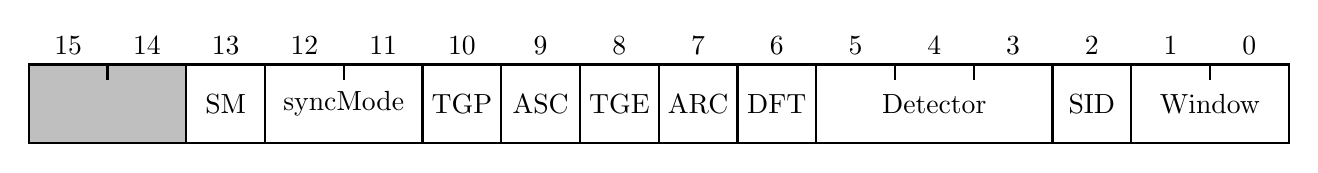
\begin{tikzpicture}
\bitrect{16}{16-\bit}
\robits{0}{2}{}
\rwbits{2}{1}{SM}
\rwbits{3}{2}{syncMode}
\rwbits{5}{1}{TGP}
\rwbits{6}{1}{ASC}
\rwbits{7}{1}{TGE}
\rwbits{8}{1}{ARC}
\rwbits{9}{1}{DFT}
\rwbits{10}{3}{Detector}
\rwbits{13}{1}{SID}
\rwbits{14}{2}{Window}
\end{tikzpicture}
\end{center}
\begin{itemize}
\item \textbf{SM:} Sync Master. Must be set to 1 at exactly one device when multiple devices are synchronized. Set to 0 when synchronization is disabled.
\item \textbf{syncMode:} Synchronization mode when multiple devices are used together
\begin{center}
\begin{tabular}{ c|c }
Setting & Synchronization\\
 \hline
00 & Disabled \\
01 & USB\\
10 & External reference\\
11 & External trigger\\
\end{tabular}
\end{center}
\item \textbf{TGP:} Tracking generator port. Set to 1 for port 2. Set to 0 for port 1.
\item \textbf{ASC:} Apply source amplitude corrections. If enabled, the amplitude calibration is used to reach better accuracy of the tracking generator output.
\item \textbf{TGE:} Tracking generator enable.
\item \textbf{ARC:} Apply receiver amplitude corrections. If enabled, the amplitude calibration is used to reach better measurement accuracy.
\item \textbf{DFT:} Use DFT to speed up the acquisition. Can not be used when the tracking generator is enabled. Only useful for low resolution bandwidths.
\item \textbf{Detector:}
\begin{center}
\begin{tabular}{ c|c }
Setting & Detector type\\
 \hline
0 & Positive peak \\
1 & Negative peak \\
2 & Sample \\
3 & Normal \\
4 & Average \\
\end{tabular}
\end{center}
\item \textbf{SID:} Signal ID enable.
\item \textbf{Window:}
\begin{center}
\begin{tabular}{ c|c }
Setting & Window\\
 \hline
0 & None \\
1 & Kaiser\\
2 & Hann\\
3 & Flattop\\
\end{tabular}
\end{center}
\end{itemize}


\subsection{SpectrumAnalyzerResult}
This packet is transmitted by the LibreVNA for every point in the sweep when in spectrum analyzer mode.

The packet contains the following fields:
\begin{ThreePartTable}
\setlength\tabcolsep{3pt}

\begin{longtable}{p{0.08\textwidth} |  p{0.08\textwidth}  |  p{0.1\textwidth}| p{0.25\textwidth} | p{0.43\textwidth}}
\toprule
\textbf{Offset} &\textbf{Length} &\textbf{Type} & \textbf{Name} &\textbf{Description} \\ 
\hline
\endhead
\midrule[\heavyrulewidth]
\endfoot  
\midrule[\heavyrulewidth]
%\insertTableNotes  % tell LaTeX where to insert the table-related notes
\endlastfoot

0 & 4 & FLOAT & Port 1 & Signal level in mW at port 1 \\
4 & 4 & FLOAT & Port 2 & Signal level in mW at port 2 \\
8 & 8 & UINT64 & Frequency/Time & Frequency of the point (or time since beginning of SA mode if in zerospan) \\
16 & 2 & UINT16 & PointNum & Number of the point in the sweep \\
\end{longtable}   
\end{ThreePartTable}

\subsection{Nack}
This packet is used to make the device send the DeviceInfo packet. It has no payload.

\subsection{RequestSourceCal}
This packet is used to make the device send the source amplitude calibration. It has no payload. For each source amplitude calibration point one SourceCalPoint packet will be returned.

\subsection{RequestSourceCal}
This packet is used to make the device send the receiver amplitude calibration. It has no payload. For each receiver amplitude calibration point one ReceiverCalPoint packet will be returned.

\subsection{SourceCalPoint}
This packet contains one source calibration point. It can be transmitted in both directions. When reading the source calibration, it is transmitted from the device to the host. When writing the source calibration multiple of these packets are transferred from the host to the device. In both cases the packet for the point with the highest point number must be transmitted last.

The packet contains the following fields:
\begin{ThreePartTable}
\setlength\tabcolsep{3pt}

\begin{longtable}{p{0.08\textwidth} |  p{0.08\textwidth}  |  p{0.1\textwidth}| p{0.25\textwidth} | p{0.43\textwidth}}
\toprule
\textbf{Offset} &\textbf{Length} &\textbf{Type} & \textbf{Name} &\textbf{Description} \\ 
\hline
\endhead
\midrule[\heavyrulewidth]
\endfoot  
\midrule[\heavyrulewidth]
%\insertTableNotes  % tell LaTeX where to insert the table-related notes
\endlastfoot

0 & 1 & UINT8 & TotalPoints & Amount of total points in the amplitude calibration \\
1 & 1 & UINT8 & PointNum & Number of the calibration point contained in this packet \\
2 & 4 & UINT32 & Frequency & Frequency of the calibration point in \SI{10}{\hertz} \\
6 & 2 & INT16 & Port 1 & Correction value for port 1 in $\frac{1}{100}$dB \\
8 & 2 & INT16 & Port 2 & Correction value for port 2 in $\frac{1}{100}$dB \\
\end{longtable}   
\end{ThreePartTable}

\subsection{ReceiverCalPoint}
This packet contains one receiver calibration point. It can be transmitted in both directions. When reading the receiver calibration, it is transmitted from the device to the host. When writing the receiver calibration multiple of these packets are transferred from the host to the device. In both cases the packet for the point with the highest point number must be transmitted last.

The packet payload is identical to the SourceCalPoint packet.

\subsection{SetIdle}
This packet is used to stop any data acquisition from the LibreVNA. It has no payload.

\subsection{RequestFrequencyCorrection}
This packet is used to make the device send the FrequencyCorrection packet. It has no payload.

\subsection{FrequencyCorrection}
This packet contains the frequency correction factor for the internal reference. It can be transmitted in both directions. When reading the frequency correction, it is transmitted from the device to the host. When writing the frequency correction, it is transmitted from the host to the device.

The packet contains the following fields:
\begin{ThreePartTable}
\setlength\tabcolsep{3pt}

\begin{longtable}{p{0.08\textwidth} |  p{0.08\textwidth}  |  p{0.1\textwidth}| p{0.25\textwidth} | p{0.43\textwidth}}
\toprule
\textbf{Offset} &\textbf{Length} &\textbf{Type} & \textbf{Name} &\textbf{Description} \\ 
\hline
\endhead
\midrule[\heavyrulewidth]
\endfoot  
\midrule[\heavyrulewidth]
%\insertTableNotes  % tell LaTeX where to insert the table-related notes
\endlastfoot

0 & 4 & FLOAT & PPM & Error of the internal TCXO in ppm \\
\end{longtable}   
\end{ThreePartTable}

\subsection{RequestAcquisitionFrequencySettings}
This packet is used to make the device send the AcquisitionFrequencySettings packet. It has no payload.

\subsection{AcquisitionFrequencySettings}
This packet contains the configuration of the acquisition hardware. These settings are at default values after the device has booted. It is normally not required to send this packet but changing these settings might be useful in special use cases. It can be transmitted in both directions. When reading the acquisition settings, it is transmitted from the device to the host. When writing the acquisition settings, it is transmitted from the host to the device.

The packet contains the following fields:
\begin{ThreePartTable}
\setlength\tabcolsep{3pt}

\begin{longtable}{p{0.08\textwidth} |  p{0.08\textwidth}  |  p{0.1\textwidth}| p{0.25\textwidth} | p{0.43\textwidth}}
\toprule
\textbf{Offset} &\textbf{Length} &\textbf{Type} & \textbf{Name} &\textbf{Description} \\ 
\hline
\endhead
\midrule[\heavyrulewidth]
\endfoot  
\midrule[\heavyrulewidth]
%\insertTableNotes  % tell LaTeX where to insert the table-related notes
\endlastfoot

0 & 4 & UINT32 & 1.IF frequency & 1.IF frequency in Hz \\
4 & 1 & UINT8 & ADC prescaler & Prescaler used for the ADC sampling (refer to the FPGA protocol) \\
5 & 2 & UINT16 & DFT phase increment & Phase increment of the DFT between ADC samples (refer to the FPGA protocol). Together with the ADC prescaler it also sets the 2.IF frequency. \\
\end{longtable}   
\end{ThreePartTable}

\subsection{DeviceStatusV1}
This packet contains the status of the device. It can be requested by sending a RequestDeviceStatus packet. The device also sends this packet on its own. The interval in which this packet is sent depends on the currently active mode.

The packet contains the following fields:
\begin{ThreePartTable}
\setlength\tabcolsep{3pt}

\begin{longtable}{p{0.08\textwidth} |  p{0.08\textwidth}  |  p{0.1\textwidth}| p{0.25\textwidth} | p{0.43\textwidth}}
\toprule
\textbf{Offset} &\textbf{Length} &\textbf{Type} & \textbf{Name} &\textbf{Description} \\ 
\hline
\endhead
\midrule[\heavyrulewidth]
\endfoot  
\midrule[\heavyrulewidth]
%\insertTableNotes  % tell LaTeX where to insert the table-related notes
\endlastfoot

0 & 1 & UINT8 & StatusBits & Bitmap of various states. See below.\\
1 & 1 & UINT8 & temp\_source & Temperature of the source PLL in \si{\celsius} \\
2 & 1 & UINT8 & temp\_LO1 & Temperature of the 1.LO PLL in \si{\celsius} \\
3 & 1 & UINT8 & temp\_MCU & Temperature of the microcontroller in \si{\celsius} \\
\end{longtable}   
\end{ThreePartTable}

\paragraph{StatusBits:}
\begin{center}
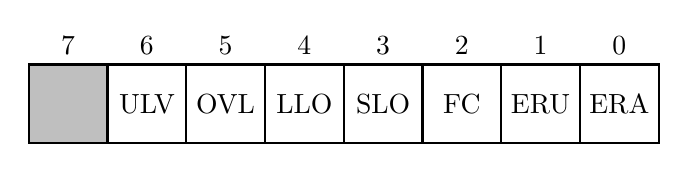
\begin{tikzpicture}
\bitrect{8}{8-\bit}
\robits{0}{1}{}
\rwbits{1}{1}{ULV}
\rwbits{2}{1}{OVL}
\rwbits{3}{1}{LLO}
\rwbits{4}{1}{SLO}
\rwbits{5}{1}{FC}
\rwbits{6}{1}{ERU}
\rwbits{7}{1}{ERA}
\end{tikzpicture}
\end{center}
\begin{itemize}
\item \textbf{ULV:} Unlevel. The requested output signal amplitude can not be reached. This is not actually measured and based on calculations only.
\item \textbf{OVL:} ADC overload. The amplitude of at least one of the ADCs reached the non-linear region and the signal level can not be trusted.
\item \textbf{LLO:} 1.LO locked.
\item \textbf{SLO:} Source locked.
\item \textbf{FC:} FPGA successfully configured.
\item \textbf{ERU:} External reference used. The external reference input is used for all PLLs.
\item \textbf{ERA:} External reference available. A signal is detected at the external reference input.
\end{itemize}

\subsection{RequestDeviceStatus}
This packet is used to make the device send the DeviceStatusV1 packet. It has no payload.

\subsection{VNADatapoint}
The VNADatapoint packet is generated by the device for every completed sweep point when in VNA mode.
\begin{important}
This packet has the CRC set to 0x00000000 as the CRC calculation would take too long when using high IF bandwidths.
\end{important}

The packet contains the following fields:
\begin{ThreePartTable}
\setlength\tabcolsep{3pt}

\begin{longtable}{p{0.08\textwidth} |  p{0.08\textwidth}  |  p{0.1\textwidth}| p{0.25\textwidth} | p{0.43\textwidth}}
\toprule
\textbf{Offset} &\textbf{Length} &\textbf{Type} & \textbf{Name} &\textbf{Description} \\ 
\hline
\endhead
\midrule[\heavyrulewidth]
\endfoot  
\midrule[\heavyrulewidth]
%\insertTableNotes  % tell LaTeX where to insert the table-related notes
\endlastfoot

0 & 8 & UINT64 & Frequency & Frequency of the sweep point in Hz\\
8 & 2 & INT16 & PowerLevel & Stimulus level of the sweep point in $\frac{1}{100}$dBm \\
10 & 2 & UINT16 & PointNumber & Number of this point in the sweep \\
12 & 4*x & Array of FLOAT & Real values & The real parts of a variable amount of receiver data \\
12+4*x & 4*x & Array of FLOAT & Imag values & The imaginary parts of a variable amount of receiver data \\
12+8*x & 1*x & UINT8 & Array of UINT8 & Variable data description \\
\end{longtable}   
\end{ThreePartTable}

The sampling data consists of a variable amount of values. The amount of values depend on the amount of configured stages and also on the hardware architecture (might change in the future). The VNADatapoint contains three arrays of equal length. Two of the arrays contain the real and imaginary parts of the acquired data. The third array contains a bitmask for every value, describing the content. The length of all arrays is not explicitly transmitted and must be inferred from the overall packet length.


\paragraph{Data description bitmask:}
\begin{center}
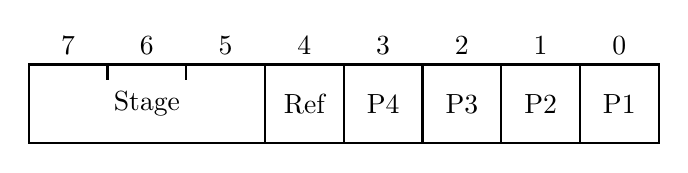
\begin{tikzpicture}
\bitrect{8}{8-\bit}
\rwbits{0}{3}{Stage}
\rwbits{3}{1}{Ref}
\rwbits{4}{1}{P4}
\rwbits{5}{1}{P3}
\rwbits{6}{1}{P2}
\rwbits{7}{1}{P1}
\end{tikzpicture}
\end{center}
\begin{itemize}
\item \textbf{Stage:} The active stage when the value was acquired. The port on which the stimulus was active during this stage is known from the SweepSettings packet that was used to set up the currently active sweep.
\item \textbf{Ref:} The value is from a reference receiver.
\item \textbf{P4:} The value is from a port 4 receiver.
\item \textbf{P3:} The value is from a port 3 receiver.
\item \textbf{P2:} The value is from a port 2 receiver.
\item \textbf{P1:} The value is from a port 1 receiver.
\end{itemize}
As the LibreVNA 1.0 only has two ports, P3 and P4 are never used and reserved for future developments.

In case of a three receiver architecture (as the LibreVNA 1.0 has), multiple port bits can be set for reference receiver values. For a typical full two-port sweep, the LibreVNA 1.0 will generate six values for every sweep point:
\begin{ThreePartTable}
\setlength\tabcolsep{3pt}

\begin{longtable}{p{0.08\textwidth} |  p{0.1\textwidth}  |  p{0.6\textwidth}}
\toprule
\textbf{\#} &\textbf{Bitmask} &\textbf{Content} \\ 
\hline
\endhead
\midrule[\heavyrulewidth]
\endfoot  
\midrule[\heavyrulewidth]
%\insertTableNotes  % tell LaTeX where to insert the table-related notes
\endlastfoot

1 & 0x01 & Port 1 receiver signal during stage 0 \\
2 & 0x02 & Port 2 receiver signal during stage 0 \\
3 & 0x13 & Reference receiver signal during stage 0 \\
4 & 0x21 & Port 1 receiver signal during stage 1 \\
5 & 0x22 & Port 2 receiver signal during stage 1 \\
6 & 0x33 & Reference receiver signal during stage 1 \\
\end{longtable}   
\end{ThreePartTable}


\subsection{SetTrigger}
This packet is used when multiple devices are synchronized over USB and can be transmitted in both directions. It has no payload. Synchronized devices must be logically organized in a closed loop. When a SetTrigger packet is received from any devices in the loop it must be passed on to the next device in the loop.

\subsection{ClearTrigger}
This packet is used when multiple devices are synchronized over USB and can be transmitted in both directions. It has no payload. Synchronized devices must be logically organized in a closed loop. When a ClearTrigger packet is received from any devices in the loop it must be passed on to the next device in the loop.

\end{document}
